\begin{figure}[ht]
    \centering


\tikzset{every picture/.style={line width=0.75pt}} %set default line width to 0.75pt

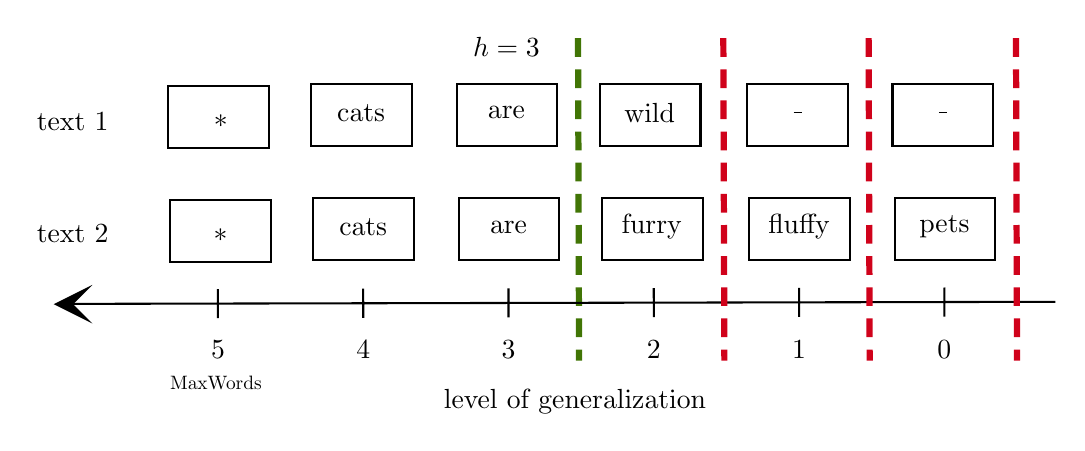
\begin{tikzpicture}[x=0.75pt,y=0.75pt,yscale=-1,xscale=1]
%uncomment if require: \path (0,316); %set diagram left start at 0, and has height of 316

%Shape: Rectangle [id:dp5153514125810188]
\draw   (210,42) -- (258.5,42) -- (258.5,72) -- (210,72) -- cycle ;

%Shape: Rectangle [id:dp3792357730299869]
\draw   (280,42) -- (328.5,42) -- (328.5,72) -- (280,72) -- cycle ;

%Shape: Rectangle [id:dp5360715303240602]
\draw   (349,42) -- (397.5,42) -- (397.5,72) -- (349,72) -- cycle ;

%Shape: Rectangle [id:dp39881760222299123]
\draw   (420,42) -- (468.5,42) -- (468.5,72) -- (420,72) -- cycle ;

%Shape: Rectangle [id:dp24969521881010048]
\draw   (490,42) -- (538.5,42) -- (538.5,72) -- (490,72) -- cycle ;

%Shape: Rectangle [id:dp1737030576273597]
\draw   (211,97) -- (259.5,97) -- (259.5,127) -- (211,127) -- cycle ;

%Shape: Rectangle [id:dp2321963000324494]
\draw   (281,97) -- (329.5,97) -- (329.5,127) -- (281,127) -- cycle ;

%Shape: Rectangle [id:dp6988583402431512]
\draw   (350,97) -- (398.5,97) -- (398.5,127) -- (350,127) -- cycle ;

%Shape: Rectangle [id:dp7718120947102272]
\draw  [fill={rgb, 255:red, 255; green, 255; blue, 255 }  ,fill opacity=1 ] (421,97) -- (469.5,97) -- (469.5,127) -- (421,127) -- cycle ;

%Shape: Rectangle [id:dp4373041939092148]
\draw  [fill={rgb, 255:red, 255; green, 255; blue, 255 }  ,fill opacity=1 ] (491,97) -- (539.5,97) -- (539.5,127) -- (491,127) -- cycle ;

%Shape: Rectangle [id:dp7370656893447207]
\draw   (141,43) -- (189.5,43) -- (189.5,73) -- (141,73) -- cycle ;
%Shape: Rectangle [id:dp45288136830178805]
\draw   (142,98) -- (190.5,98) -- (190.5,128) -- (142,128) -- cycle ;
%Straight Lines [id:da8313945580724125]
\draw [color={rgb, 255:red, 65; green, 117; blue, 5 }  ,draw opacity=1 ][line width=2.25]  [dash pattern={on 6.75pt off 4.5pt}]  (338.5,20) -- (339,175.33) ;


%Straight Lines [id:da846675768790583]
\draw    (95,148) -- (568.5,147) (164.99,140.85) -- (165.01,154.85)(234.98,140.7) -- (235.01,154.7)(304.98,140.56) -- (305.01,154.56)(374.98,140.41) -- (375.01,154.41)(444.98,140.26) -- (445.01,154.26)(514.98,140.11) -- (515.01,154.11) ;


\draw  [fill={rgb, 255:red, 0; green, 0; blue, 0 }  ,fill opacity=1 ] (102,155.67) -- (87,148.17) -- (102,140.67) -- (94.5,148.17) -- cycle ;
%Straight Lines [id:da7170976620765326]
\draw [color={rgb, 255:red, 208; green, 2; blue, 27 }  ,draw opacity=1 ][line width=2.25]  [dash pattern={on 6.75pt off 4.5pt}]  (408.5,20) -- (409,175.33) ;


%Straight Lines [id:da920755443743104]
\draw [color={rgb, 255:red, 208; green, 2; blue, 27 }  ,draw opacity=1 ][line width=2.25]  [dash pattern={on 6.75pt off 4.5pt}]  (478.5,20) -- (479,175.33) ;


%Straight Lines [id:da6869452406118943]
\draw [color={rgb, 255:red, 208; green, 2; blue, 27 }  ,draw opacity=1 ][line width=2.25]  [dash pattern={on 6.75pt off 4.5pt}]  (549.5,20) -- (550,175.33) ;



% Text Node
\draw (304,56) node  [align=left] {are};
% Text Node
\draw (234,56) node  [align=left] {cats};
% Text Node
\draw (373,56) node  [align=left] {wild};
% Text Node
\draw (444,56) node  [align=left] {\_};
% Text Node
\draw (514,56) node  [align=left] {\_};
% Text Node
\draw (515,111) node  [align=left] {pets};
% Text Node
\draw (445,111) node  [align=left] {fluffy};
% Text Node
\draw (374,111) node  [align=left] {furry};
% Text Node
\draw (305,111) node  [align=left] {are};
% Text Node
\draw (235,111) node  [align=left] {cats};
% Text Node
\draw (337,195) node  [align=left] {level of generalization};
% Text Node
\draw (235,170) node  [align=left] {4};
% Text Node
\draw (305,170) node  [align=left] {3};
% Text Node
\draw (375,170) node  [align=left] {2};
% Text Node
\draw (445,170) node  [align=left] {1};
% Text Node
\draw (515,170) node  [align=left] {0};
% Text Node
\draw (165,170) node  [align=left] {5};
% Text Node
\draw (166.25,117) node  [align=left] {*};
% Text Node
\draw (166.33,62) node  [align=left] {*};
% Text Node
\draw (95,60) node  [align=left] {text 1};
% Text Node
\draw (95,114) node  [align=left] {text 2};
% Text Node
\draw (304,24) node  [align=left] {$\displaystyle h=3$};
% Text Node
\draw (164,186) node [scale=0.7] [align=left] {MaxWords};


\end{tikzpicture}

    \caption{Prefix generalizer (h=3)}\label{fig:prefix_generalizer_1}
\end{figure}